\documentclass[preview]{standalone}
\usepackage[usenames]{color}
\usepackage{tikz}
\usepackage{color}
\usepackage{listings}
\usetikzlibrary{shapes,arrows,shadows,decorations,decorations.text}

\newcommand{\lorem}[0]{Lorem ipsum dolor sit amet, consectetuer
  adipiscing elit. Donec hendrerit tempor tellus. Donec pretium
  posuere tellus. Proin quam nisl, tincidunt et, mattis eget,
  convallis nec, purus. Cum sociis natoque penatibus et magnis dis
  parturient montes, nascetur ridiculus mus. Nulla posuere. Donec
  vitae dolor. Nullam tristique diam non turpis. Cras placerat
  accumsan nulla. Nullam rutrum. Nam vestibulum accumsan nisl.}

\newcommand{\asm}[0]{start: popl \%eax popl \%eax movl \$0, \%esi
  movl \$10, \%edx jmp read_arg read_arg: popl \%eax cmpl \$0,
  \%eax je sort movl \$0, \%edi movl \$0, \%ecx store_arg: movl
  \%ecx, lst(,\%esi,4) incl \%esi read_ch: movb 0(\%eax,\%edi),
  \%bl cmpl \$0, \%ebx je store_arg imul \%edx, \%ecx subl \$48,
  \%ebx addl \%ebx, \%ecx incl \%edi jmp read_ch}

\begin{document}
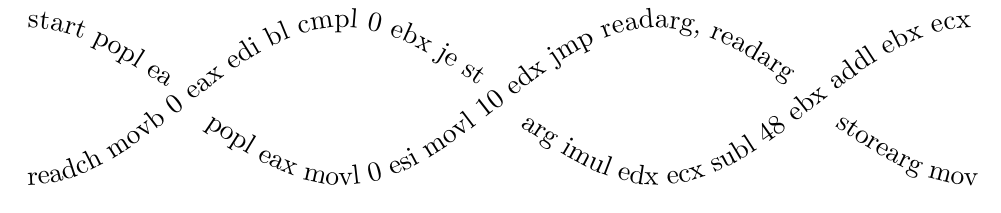
\begin{tikzpicture}
    \path [decorate, decoration={text along path, text={start popl eax}}]
    (0,1) cos (1.75,0.25);

    \path [decorate, decoration={text along path, text={popl eax movl 0 esi movl 10 edx jmp readarg, readarg popl}}]
    (2.25,-0.25) sin (4,-1) cos (6,0) sin (8,1) cos (9.75,0.25);

    \path [decorate, decoration={text along path, text={readch movb 0 eax edi bl cmpl 0 ebx je storearg}}]
    (0,-1) cos (2,0) sin (4,1) cos (5.75,0.25);

    \path [decorate, decoration={text along path, text={arg imul edx ecx subl 48 ebx addl ebx ecx incl edi jmp readch}}]
    (6.25,-0.25) sin (8,-1) cos (10,0) sin (12,1);

    \path [decorate, decoration={text along path, text={storearg movl ecx lst esi 4 incl esi}}]
    (10.25,-0.25) sin (12,-1);
\end{tikzpicture}
\end{document}

% start:; popl %eax; popl %eax movl $0, %esi; movl $10, %edx; jmp read_arg
% read_arg:; popl %eax; cmpl $0, %eax; je sort; movl $0, %edi; movl $0, %ecx
% store_arg:; movl %ecx, lst(,%esi,4); incl %esi
% read_ch:; movb 0(%eax,%edi), %bl; cmpl $0, %ebx; je store_arg; imul %edx, %ecx; subl $48, %ebx; addl %ebx, %ecx; incl %edi; jmp read_ch
